\documentclass[conference]{IEEEtran}
\IEEEoverridecommandlockouts
% The preceding line is only needed to identify funding in the first footnote. If that is unneeded, please comment it out.
\usepackage{amsmath,amssymb,amsfonts}
\usepackage{cite}
\usepackage{algorithmic}
\usepackage{graphicx}
\usepackage{textcomp}
\usepackage{xcolor}
\usepackage{booktabs}
\usepackage{float}
\def\BibTeX{\textrm{B \kern -.05em \textsc{i \kern -.025em b} \kern -.08em
T \kern -.1667em \lower .7ex \hbox{E} \kern -.125emX}}
\begin{document}

\title{Helix Requirements Management\\

}

\author{
    \IEEEauthorblockN{Kévyn Marins}
    \IEEEauthorblockA{
        \textit{Faculty of Engineering} \\
        \textit{University of Porto}\\
        Porto, Portugal \\
        up201902398@up.pt
    }
    \and
    \IEEEauthorblockN{Nuno Fernandes}
    \IEEEauthorblockA{
        \textit{Faculty of Engineering} \\
        \textit{University of Porto}\\
        Porto, Portugal \\
        up202403077@up.pt
    }
    \and
    \IEEEauthorblockN{Rui Soares}
    \IEEEauthorblockA{
        \textit{Faculty of Engineering} \\
        \textit{University of Porto}\\
        Porto, Portugal \\
        up202103631@up.pt
    }
    \and
    \IEEEauthorblockN{Simão Antunes}
    \IEEEauthorblockA{
        \textit{Faculty of Engineering} \\
        \textit{University of Porto}\\
        Porto, Portugal \\
        up202403111@up.pt
    }
}

\maketitle

\begin{abstract}
Requirements management ensures that stakeholder objectives are consistent with the project's final results.
HelixRM offers a comprehensive solution for tracking, evaluating, deconstructing, and prioritizing requirements.
This paper investigates how HelixRM enhances collaboration, traceability, and adaptability in requirements management while integrating with widely utilized development tools.
\end{abstract}

\begin{IEEEkeywords}
Requirements Management, HelixRM, Traceability, Collaboration, Project Development
\end{IEEEkeywords}

\section{Introduction}\label{sec:introduction}
Requirements management is an essential aspect of effective project development, as it guarantees that stakeholder needs and objectives are clearly articulated, recorded, and tracked during the project lifecycle.
Proper requirements management minimizes the risk of scope creep, misunderstandings, and unmet goals, all of which can greatly affect project success.

HelixRM supports this process by providing a centralized platform for managing and decomposing requirements into actionable specifications.
With features like hierarchical organization, traceability, version control, and integration with tools such as Jira, HelixRM improves collaboration among stakeholders and guarantees that requirements align with business objectives.
Its functionalities empower teams to quickly respond to changes, maintain consistency, and enhance project transparency, making it an invaluable tool for overseeing complex or large-scale projects.

\section{Functionalities of HelixRM}\label{sec:functionalities-of-helixrm}

\section{Features}

\subsection{Track Requirements}

Helix RM's Requirement Tracking feature is essential for keeping
track of the software needs of any project.
It helps to maintain requirements clear, connected to
deliverables, and tracked against their fulfilment criteria.

With a defined plan for managing the requirements,which
are essential to maintaining the project's high quality and
making sure it satisfies the expectations of the stakeholders,
such an organised approach improves project management.

\begin{itemize}
    \item Why Track Requirements
    \begin{itemize}
        \item Defined needs: Requirements are clear descriptions of a specific software product\cite{b1}.
        \item Completion Criteria: More precise measurements for when a need is met\cite{b2}.
    \end{itemize}

    \item Advantages of Monitoring Requirements
    \begin{itemize}
        \item Enhanced Cooperation: User-centred design concepts, enhancing personalisation to satisfy requirements\cite{b3}.
        \item Better Project Metrics: Structure for examining how needs have changed over time, for well-informed decision-making\cite{b2}.
    \end{itemize}

    \item Real World Usage
    \begin{itemize}
        \item Software Development: Used in multiple software projects, in order to monitor and address criteria in order to produce higher-quality results\cite{b4}.
        \item Product lifetime Management: Easier to include requirement management into more comprehensive processes for the product lifetime\cite{b3}.
    \end{itemize}
\end{itemize}

Even while it might be very advantageous, it might be
argued that the extra difficulty of managing all those needs
could just result in increased costs and possibly create project
timeline delays.
For most people, striking a balance between meticulous
tracking and nimble approaches is never easy.


\subsection{Review Requirements}\label{subsec:review-requirements2}
Receiving feedback about the requirements is an important step 
of the management process because it helps ensure the requirements 
are clear and aligned with the scope of the project. 
Helix offers features to help streamline this process.

\subsubsection{Review Mode View}
The Review Mode View is the centre point where users 
can review and comment on requirements.
When users open
a requirement document, they are presented with a hierarchical 
document where they can perform activities related to the review 
process, like adding notes~\cite{perforce_2024}.
The image Figure~\ref{fig:review_mode} shows the Review Mode View, with an example of a requirement.

\begin{figure}[htbp]
    \centering
    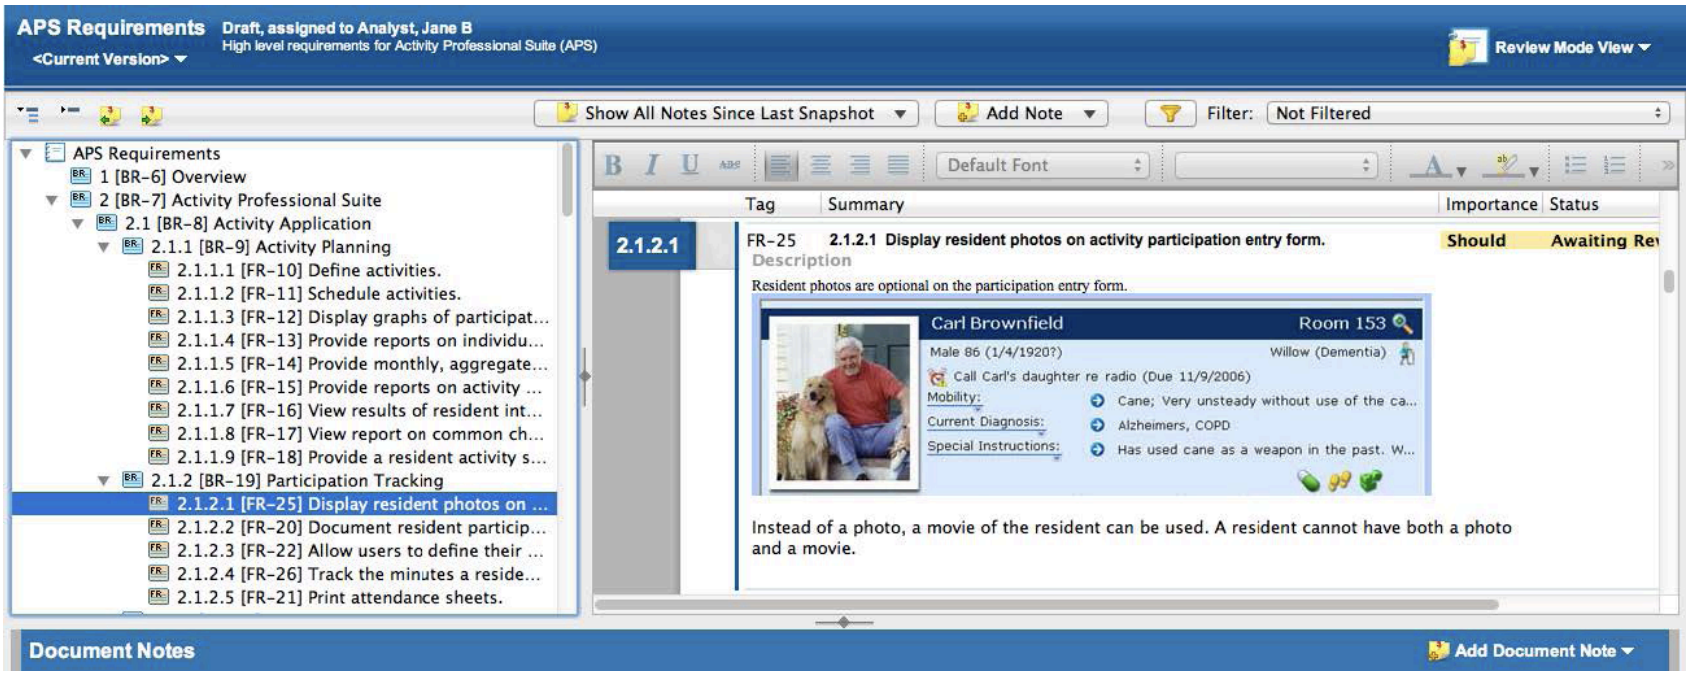
\includegraphics[width=\linewidth]{images/review-mode-view}
    \caption{Helix review mode view.}
    \label{fig:review_mode}
\end{figure}

\subsubsection{Review Feedback}
As part of the process of requirement review, 
Helix gives users the options to add review notes, 
email feedback, or directly edit the requirements.

\paragraph{Review Notes}
Users can add review notes to specific requirements to give 
feedback or ask for changes.
The notes are displayed in
line with the requirements, making it possible to have a 
thread of all feedback given for a requirement~\cite{perforce_2024}.
The image Figure~\ref{fig:review_notes} shows an example of a note left in a requirement.

\begin{figure}[htbp]
    \centering
    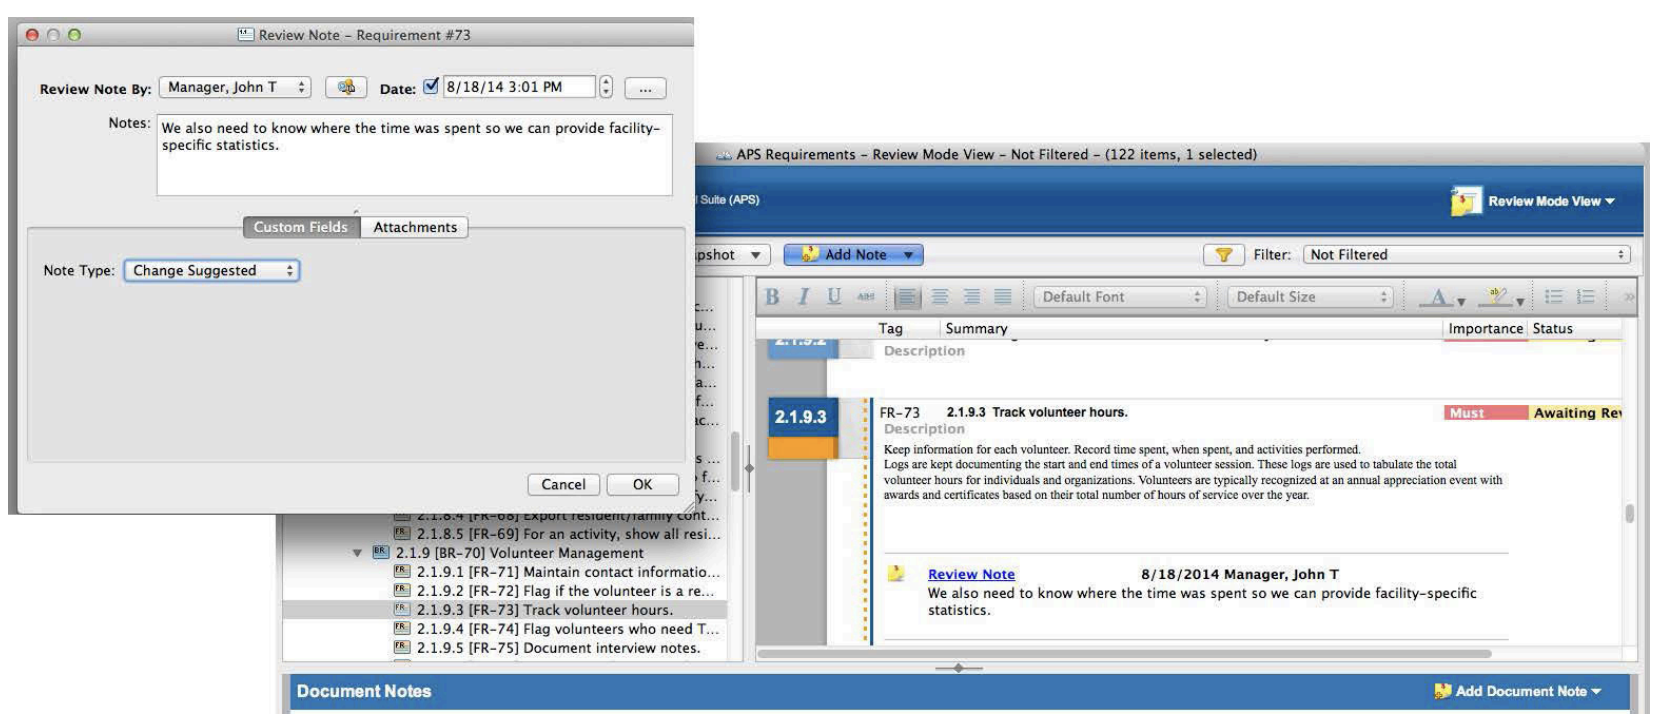
\includegraphics[width=\linewidth]{images/review-notes}
    \caption{Helix review note.}
    \label{fig:review_notes}
\end{figure}


\paragraph{Email Feedback}
Helix makes it possible to email from requirement documents to 
provide feedback.
With the enablement of email tracking,
emails and any subsequent replies are saved with the requirements, 
making it possible to track the full discussion of an item.
The image Figure~\ref{fig:review_email} shows an email panel with an example of feedback in the form of a reply~\cite{perforce_2024}.

\begin{figure}[htbp]
    \centering
    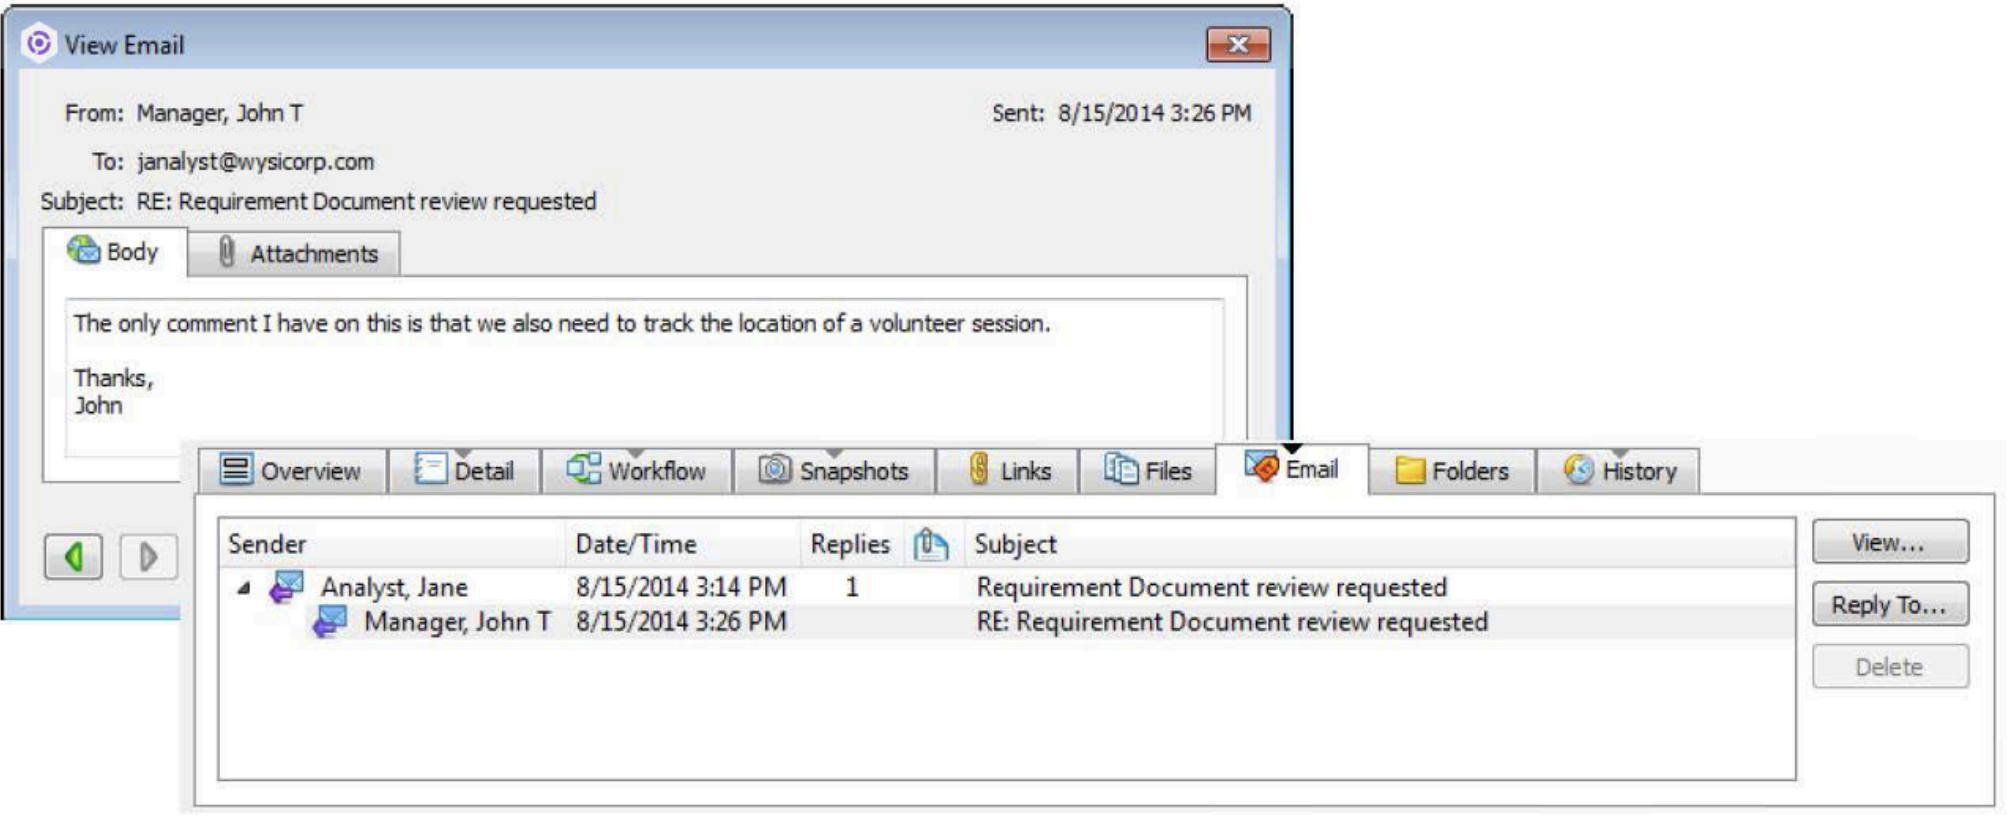
\includegraphics[width=\linewidth]{images/email-feedback}
    \caption{Helix email feedback view.}
    \label{fig:review_email}
\end{figure}

\paragraph{Edit Requirements}
There is also the option to directly change requirements, 
depending on the level of secure permissions.
Users can add a
timestamp with a name to help identify their comments or changes, 
or even apply formatting to the text to make it easier to tell them apart. 
Helix offers the possibility to create a document snapshot to help with requirement changes, 
making it possible to compare old versions with new ones.
The image Figure~\ref{fig:review_edit_feedback} shows a user adding a comment, providing  the timestamp and their name~\cite{perforce_2024}.

\begin{figure}[htbp]
    \centering
    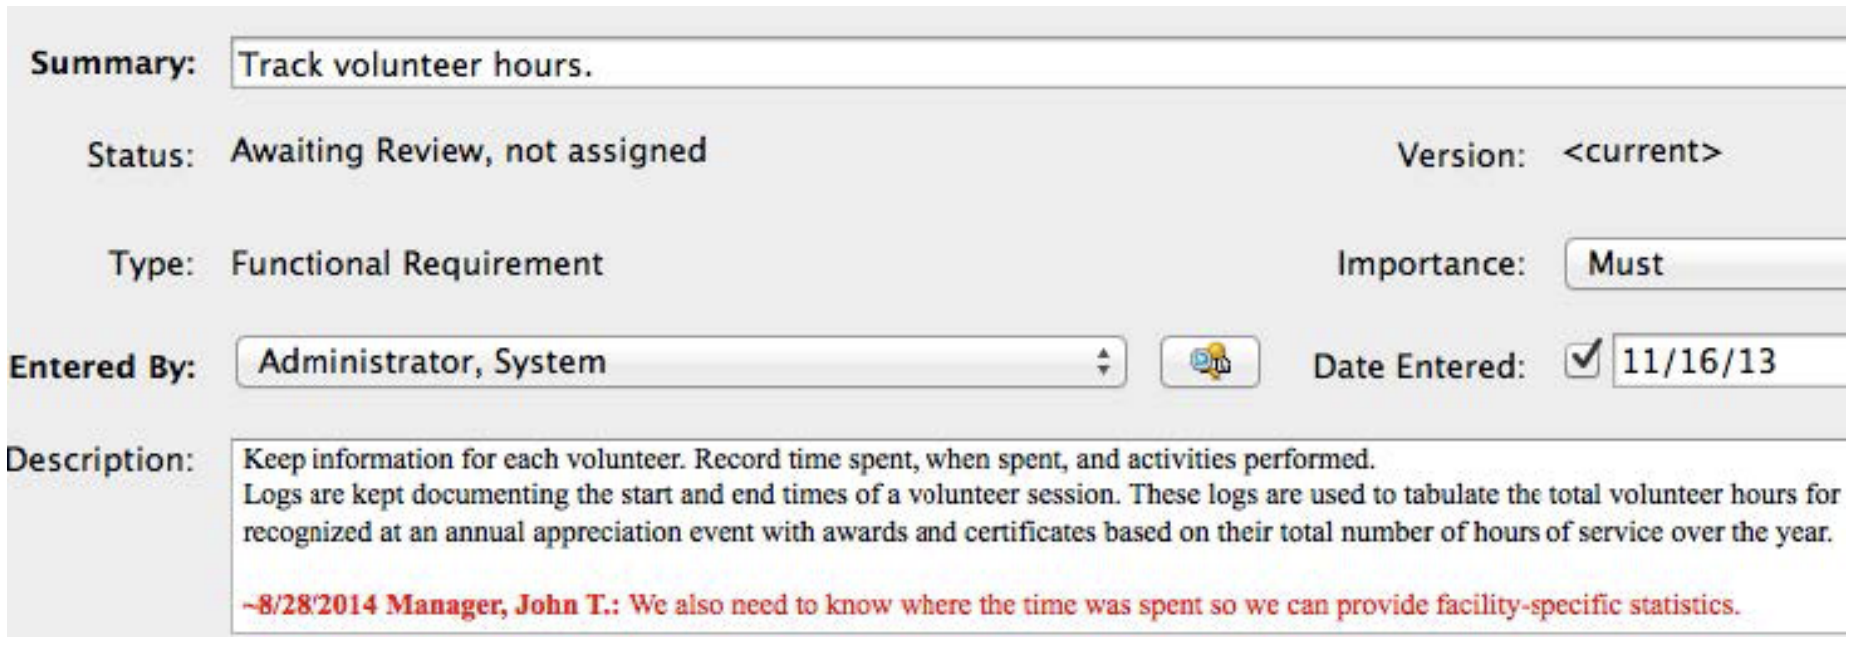
\includegraphics[width=\linewidth]{images/edit-requirements}
    \caption{Helix email feedback view.}
    \label{fig:review_edit_feedback}
\end{figure}
\subsection{Decompose Requirements}\label{subsec:decompose-requirements}

Decomposing requirements in HelixRM entails subdividing
broad business or marketing goals into specific, actionable
functional and system specifications.
This organised methodology guarantees that all elements of a
requirement are comprehensible, traceable, and manageable,
thereby optimising the development process.

\paragraph{Organize Requirements Hierarchically}
HelixRM allows users to establish and oversee hierarchical
arrangements for their requirements.
General requirements, such as “Improve user experience,” can
be further divided into more precise requirements, such as
“Ensure faster load times for pages” or “Enhance navigation intuitiveness.”
This hierarchy offers a clear visual depiction of how specific tasks
support broader objectives.

\paragraph{Create Traceability Links}
Traceability is a fundamental aspect of HelixRM, permitting
users to form direct connections between parent requirements
and their detailed sub-requirements.
For example, a business requirement can be linked to functional
specifications and related test cases.
This guarantees cohesion across all project components and
simplifies impact analysis for prospective changes.

\paragraph{Collaborate with Stakeholders}
HelixRM’s collaboration features promote smooth communication
throughout the decomposition process.
Team members and stakeholders can provide instantaneous feedback
and comments, ensuring transparency and agreement.
This engaging method minimizes ambiguity and fosters a
shared understanding of the requirements.

\paragraph{Use Templates and Reuse Requirements}
The platform improves efficiency by offering templates
and permitting the reuse of previously validated
requirements across various projects.
This not only saves time but also guarantees consistency
and adherence to organizational standards.

\paragraph{Analyze Risks and Dependencies}
As part of the decomposition process, HelixRM enables users to recognize and document potential risks and dependencies linked to particular requirements.
Integrated risk assessment tools support teams in proactively managing challenges that may arise during development.

\paragraph{Export for Wider Accessibility}
For external stakeholders or team members not directly utilizing HelixRM, decomposed requirements can be exported into widely used formats such as Word or Excel.
This feature guarantees that all pertinent parties can review, approve, or contribute to the refinement process.

By utilizing these functionalities, HelixRM ensures that intricate requirements are methodically disaggregated, fostering improved alignment, traceability, and implementation throughout the project lifecycle.

\subsection{Prioritize Requirements}

Another defining features of HelixRM is its ability to streamline and enhance the prioritization of requirements.
This functionality is designed to evaluate and rank requirements based on criteria such as business value, complexity, urgency, and risk.
By employing weighted scoring and customizable parameters, HelixRM ensures that stakeholders can make informed decisions that align with organizational goals and project constraints.

\paragraph{Establish Clear Evaluation Criteria}
HelixRM allows users to define and customize evaluation criteria to suit the unique needs of their projects.

\paragraph{Weighted Scoring}
The platform supports weighted scoring, enabling users to assign relative importance to each evaluation criterion. This feature ensures that requirements are prioritized based on their significance to the project.

\paragraph{Automated Ranking}
HelixRM automates the ranking process, generating a prioritized list of requirements based on the established evaluation criteria and weighted scores. This functionality saves time and minimizes subjectivity in the prioritization process.

\paragraph{Collaborative Decision-Making}
The platform facilitates collaborative decision-making by providing a transparent view of the prioritized requirements. Stakeholders can review, discuss, and reach a consensus on the order of implementation.

\paragraph{Scenario Analysis}
HelixRM supports scenario analysis, allowing users to evaluate the impact of different prioritization strategies on project outcomes. This feature enables stakeholders to make data-driven decisions that maximize project value.

\paragraph{Continuous Refinement}
As project requirements evolve, HelixRM enables users to continuously refine and update the prioritization of requirements. This iterative process ensures that project goals remain aligned with changing business needs.

\subsection{Jira Integration}\label{subsec:jira-integration}

The integration of HelixRM with Jira addresses the limitations of using Jira alone for managing complex requirements.
While Jira is a robust tool for tracking bugs and managing tasks, it lacks comprehensive features for requirements and test case management.
HelixRM bridges this gap by enabling seamless connectivity between requirements, test cases, and Jira issues.

    \subsubsection*{Bidirectional Linking}
    \begin{itemize}
        \item Requirements managed in HelixRM can be linked directly to Jira issues, allowing both tools to stay synchronized.
        \item Changes made in one platform are reflected in the other, ensuring consistency across teams.
    \end{itemize}

    \subsubsection*{Visibility Across Tools}
    \begin{itemize}
        \item Users can view requirements and test cases from within Jira or monitor Jira issues in HelixRM\@.
        \item This eliminates the need to switch between tools frequently, improving workflow efficiency.
    \end{itemize}

    \subsubsection*{Traceability and Reporting}
    \begin{itemize}
        \item Linking test case results to Jira issues creates traceability between testing and issue resolution.
        \item Teams can track the status of requirements and ensure compliance with project or regulatory standards.
    \end{itemize}

    \subsubsection*{Streamlined Workflow}
    \begin{itemize}
        \item Failed tests in HelixALM can automatically generate Jira issues, reducing manual effort and ensuring prompt attention to defects.
        \item Requirements can be transformed into Jira tasks, ensuring they are implemented and tracked through completion.
    \end{itemize}

    \subsubsection*{Ease of Integration}
    HelixRM’s Jira integration is designed to be user-friendly and quick to implement.
    It comes as an out-of-the-box solution with no additional costs for existing license holders of both tools.
    The setup process takes minutes, enabling teams to immediately begin leveraging the integration’s benefits without extensive configuration.

\section{Advantages of HelixRM}\label{sec:advantages-of-helixrm}
HelixRM proves to be a valuable requirements management tool for software
and system engineering projects, offering several essential features, as
previously stated.

Its ability to integrate with common documentation formats improves
usability and facilitates collaboration among various participants,
such as stakeholders and domain experts.
This, in turn, streamlines the development process and reduces communication challenges\cite{michele_zamparelli_2006}.


The following features are some of the advantages of using HelixRM in software and system engineering projects:

\paragraph{Rapid Development}
Facilitates rapid development, helping to avoid costly delays and significantly improve time to market\footnotemark[1].

\paragraph{Scalability}
Highly scalable to support evolving space systems, easy and straightforward to extend or build new HELIX applications\footnotemark[1].

\paragraph{Flexibility}
Exceptionally flexible to support extensive configuration or integration with 3rd party software\footnotemark[1].

\paragraph{Compatibility}
Compatible with both Agile and traditional methodologies\footnotemark[2].

\paragraph{Traceability}
Provides detailed reports and metrics for project monitoring\footnotemark[2].

\paragraph{Integration}
Supports integration with other tools and systems, such as JIRA\footnotemark[2].

These features end up contributing to a better project quality,
efficiency, and adaptability in development environments\cite{youngki_hong__2010}.


\footnotetext[1]{\cite{bright_ascention_2024}}~\footnotetext[2]{\cite{helix_alm_review}}







\section{Limitations of HelixRM}\label{sec:limitations-of-helixrm}
Even with the mentioned advantages, HelixRM can be inconvenient for small teams, given certain
limitations and challenges that can impact its effectiveness.

The cost of using a resource management system like HelixRM
is often an impediment for smaller organizations that probably wouldn't need
such a complete tool in the first place\cite{lydia_y__chen_2019}.

The complexity of the tool can be overwhelming for first-time users of this kind of systems,
leading to inefficiency as the user struggles with the tool's steep learning curve\cite{the_submission_infrastructure}.

Integrating HelixRM with an already existing infrastructure can be more challenging
than what is worth, as current systems may need to be adapted to accommodate the new tool,
ending up increasing complexity\cite{christian_glaschke__2015}.

It is also worth noting that the tool's pricing information is not readily available,
which can present a barrier for potential users\footnotemark[2].

Knowing all of these shortcomings is essential for organizations to make an informed decision
when considering HelixRM for their requirements management needs.


\section{Alternative Tools}\label{sec:alternative-tools}
\begin{table}[H]
    \centering
    \begin{tabular}{p{1cm}p{3.1cm}p{3.1cm}}
        \toprule
        \textbf{Tool} & \textbf{What HelixRM Has That They Don’t} & \textbf{What They Have That HelixRM Doesn’t} \\
        \midrule
        Jira & Robust requirements traceability, test case integration. & Comprehensive task tracking for Agile teams. \\
        Aha! & Detailed traceability and test case linking. & Advanced roadmapping and idea management features. \\
        Jama Connect & Simplicity and easier integration with Jira. & Industry-leading compliance and multi-level traceability. \\
        IBM DOORS & Easier to use, faster implementation. & Enterprise-grade scalability and hierarchical requirement support. \\
        Azure DevOps & Strong requirements focus with built-in traceability. & Full DevOps suite for CI/CD and version control. \\
        \bottomrule
    \end{tabular}
    \vspace{5pt}
    \caption{Comparison of HelixRM with Other Tools}
    \label{tab:helix-vs-all}
\end{table}


\section{Acknowledgment}\label{sec:acknowledgment}
The preferred spelling of the word ``acknowledgment'' in America is without
an ``e'' after the ``g''.
Avoid the stilted expression ``one of us (R. B\@.
G.) thanks $\ldots$''.
Instead, try ``R. B. G. thanks$\ldots$''.
Put sponsor acknowledgments in the unnumbered footnote on the first page.

\section*{References}

Please number citations consecutively within brackets~\cite{b1}.
The sentence punctuation follows the bracket~\cite{b2}.
Refer simply to the reference number, as in~\cite{b3}---do not use ``Ref~\cite{b3}.'' or ``reference~\cite{b3}'' except at
the beginning of a sentence: ``Reference~\cite{b3} was the first $\ldots$''

Number footnotes separately in superscripts.
Place the actual footnote at the bottom of the column in which it was cited.
Do not put footnotes in the abstract or reference list.
Use letters for table footnotes.

Unless there are six authors or more give all authors' names; do not use
``et al.''.
Papers that have not been published, even if they have been
submitted for publication, should be cited as ``unpublished''~\cite{b4}.
Papers that have been accepted for publication should be cited as ``in press''~\cite{b5}.
Capitalize only the first word in a paper title, except for proper nouns and
element symbols.

For papers published in translation journals, please give the English
citation first, followed by the original foreign-language citation~\cite{b6}.


%\begin{thebibliography}{00}
\bibitem{b1}
    J.E., Archer. (2003).
    Requirement tracking: a streamlined approach.
    doi: 10.1109/ICRE.2003.1232774

\bibitem{b2}
    Evangelos, Markopoulos., Georgios, Alexopoulos., Nikolitsa, Bouzoukou., Javier, Bilbao. (2009).
    Software project tracking metrics analysis model based on project requirements.

\bibitem{b3}
    Maria, Grazia, Violante., Enrico, Vezzetti., Marco, Alemanni. (2017).
    An integrated approach to support the Requirement Management (RM) tool customization for a collaborative scenario.
    International Journal on Interactive Design and Manufacturing (ijidem)
    doi: 10.1007/S12008-015-0266-3

\bibitem{b4}
    Edward, R., Rang., Karen, H., Thelen. (1985).
    A Requirements to Test Tracking System (RTTS).
    doi: 10.1145/320435.320548

\bibitem{b5}
    GetApp,
    "Helix RM Pricing, Features, Reviews and Alternatives."
    Available: \url{https://www.getapp.com}.
    Accessed: Nov. 2024.

\bibitem{b6}
    A2IS,
    "Helix RM Requirements Management Features."
    Available: \url{https://a2is.com/catalog/requirements-management-software/helix-rm}.
    Accessed: Nov. 2024.

\end{thebibliography}
\bibliographystyle{plain}
\bibliography{chapters/references}

\end{document}
